% ============================================================================
% DHG508 Final Design Paper & Post-Mortem (Overleaf Template)
% Lingnan University — Critical Digital History
%
% OVERLEAF SETUP:
%   1. Upload dhg508-overleaf-template.zip to Overleaf (New Project -> Upload Project)
%   2. Menu (top left) -> Compiler -> XeLaTeX
%   3. Click Recompile
% ============================================================================

\documentclass[12pt,a4paper]{article}

\usepackage{fontspec}
\newcommand{\MainLatinFont}{Times New Roman}
\newcommand{\FallbackLatinFont}{TeX Gyre Termes}
\newcommand{\MainCJKFont}{Noto Serif CJK SC}
\newcommand{\FallbackCJKFont}{FandolSong-Regular.otf}

\IfFontExistsTF{\MainLatinFont}
  {\setmainfont{\MainLatinFont}}
  {\setmainfont{\FallbackLatinFont}}

\usepackage{xeCJK}
\IfFontExistsTF{\MainCJKFont}
  {\setCJKmainfont{\MainCJKFont}}
  {\IfFontExistsTF{Songti SC}
    {\setCJKmainfont{Songti SC}}
    {\IfFontExistsTF{SimSun}
      {\setCJKmainfont{SimSun}}
      {\setCJKmainfont{\FallbackCJKFont}}}}

\usepackage[a4paper, margin=1in]{geometry}
\usepackage{setspace}
\usepackage{booktabs}
\usepackage{array}
\usepackage{graphicx}
\usepackage{csquotes}

% Chicago Manual of Style 18th ed., Notes-Bibliography (BibLaTeX + Biber)
\usepackage[notes, backend=biber, autolang=other, isbn=false]{biblatex-chicago}
\addbibresource{references.bib}

\renewcommand{\footnotesize}{\fontsize{10}{12}\selectfont}
\usepackage[hidelinks]{hyperref}

\title{\textbf{Reactive Avatar: A Transparent Real-Time Companion}\\[0.3em]
\large Design Rationale, Evidence Boundaries, and Post-Mortem}
\author{Yiyang Zhao\\Lingnan University $\cdot$ DHG508 Critical Digital History\\
\small Live URL: \url{https://reactive-avatar.pages.dev} $\cdot$ Repo: \url{https://github.com/yiyangzhao23/reactive-avatar}}
\date{25 November 2026}

\begin{document}
\maketitle

\begin{abstract}
\noindent
State in 100--150 words: your historical or cultural question, what a user does
in your project, how documented facts (\emph{据}), inferences (\emph{推断}), and
design inventions (\emph{设}) are separated, and your main takeaway.
\end{abstract}

\onehalfspacing

\section{Historical Question and Medium}

State your historical or cultural question and explain why an interactive
simulation or application is needed rather than a static essay or film.

\section{Sources and Scholarly Conversation}

Describe your primary sources and their limits (edition, translation, OCR, or
gaps).\autocite[42]{weizenbaum1966eliza} Place \verb|\autocite[page]{key}| after
punctuation to generate Chicago footnotes.\autocite[743--750]{agre1994surveillance}

Engage with \textbf{at least three scholarly works}, showing how your design
responds to their arguments.\autocite[610--611, 619]{bender2021parrots} Connect each
work to a specific part of your build.\autocite{reactiveavatar2026}

\section{Architecture and Boundaries}

Explain how data (\texttt{.csv}/\texttt{.json}), rules, UI/engine, and Cloudflare
deployment connect, and what temporal or epistemic cutoffs apply.

\begin{figure}[htbp]
  \centering
  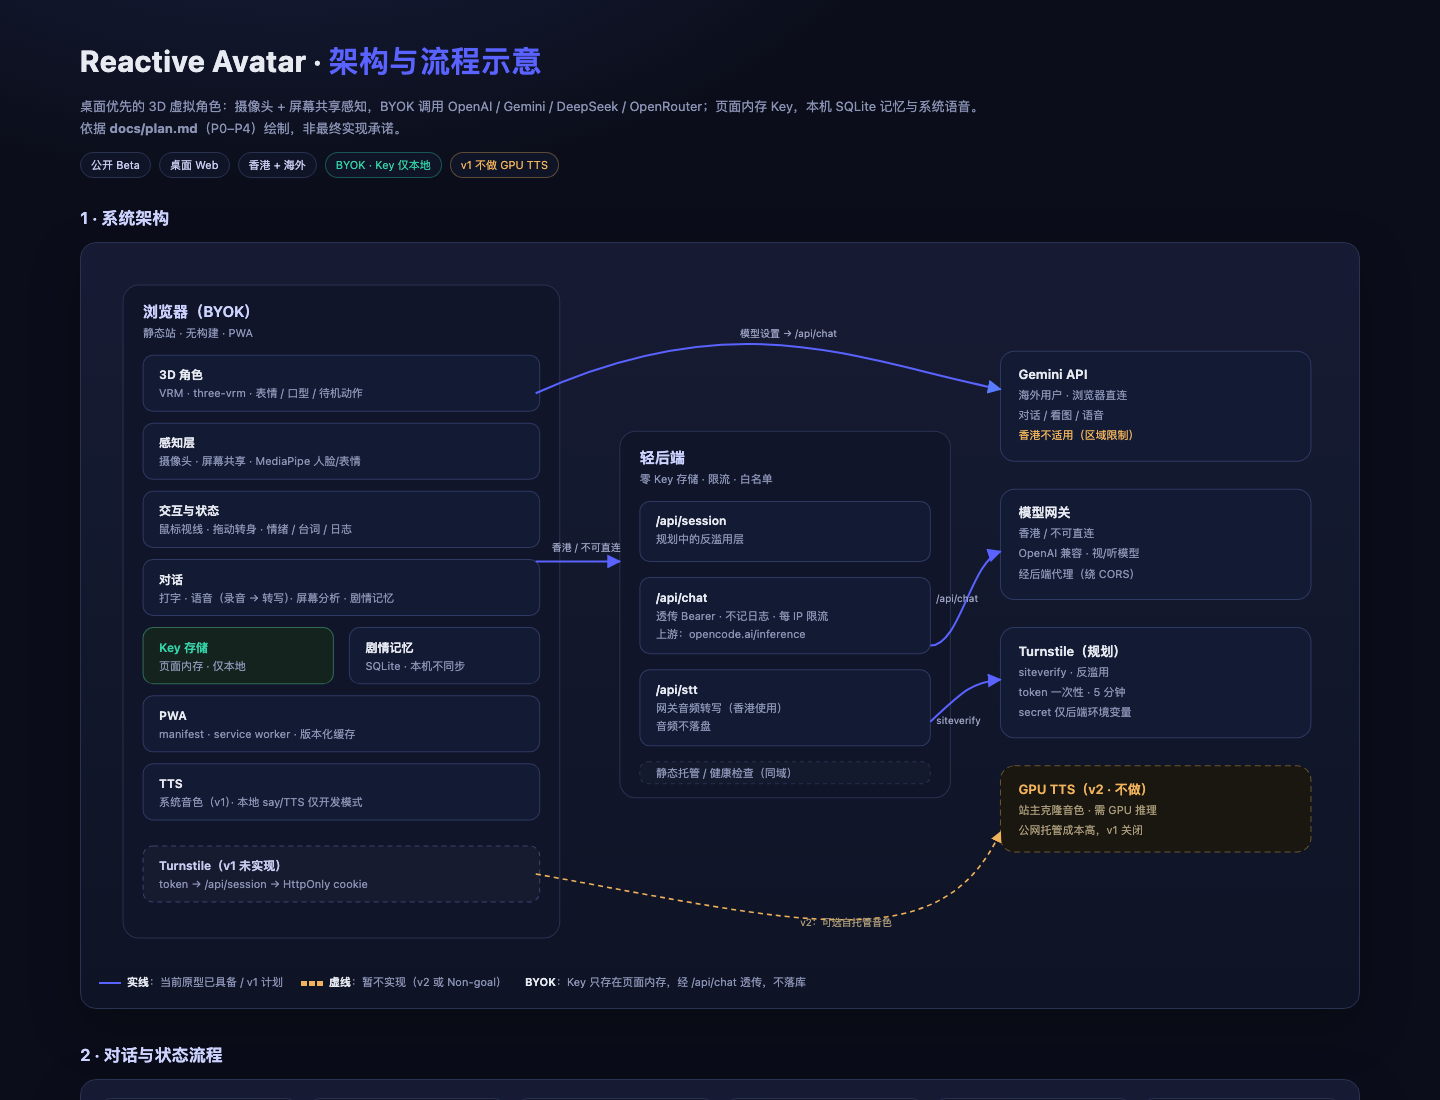
\includegraphics[width=0.92\textwidth]{schematic.png}
  \caption{Project architecture and interaction flow.}
  \label{fig:schematic}
\end{figure}

\section{Evidence Table}

Table~\ref{tab:evidence} is generated from \texttt{evidence.csv} by
\texttt{make\_evidence\_table.py}.

\begin{table}[htbp]
  \centering
  \footnotesize
  \singlespacing
  \renewcommand{\arraystretch}{1.25}
  % Auto-generated from evidence.csv by make_evidence_table.py — edit the CSV, not this file.
\begin{tabular}{p{0.27\textwidth}p{0.20\textwidth}p{0.13\textwidth}p{0.08\textwidth}p{0.22\textwidth}}
  \toprule
  \textbf{Claim / Element} & \textbf{Source / File} & \textbf{Locator} & \textbf{Level} & \textbf{Boundary / Limit} \\
  \midrule
  ELIZA makes it easy to create and maintain the illusion of understanding & Weizenbaum, ELIZA (1966) & p. 42 & 据 & Close reading of one article; this project has no user study \\
  The test of understanding is drawing valid conclusions, not continuing a conversation & Weizenbaum, ELIZA (1966) & p. 43 & 据 & A program-level claim, not a benchmark of current LLMs \\
  Capture tracks activity through a grammar and reorganizes that activity & Agre, Surveillance and Capture (1994) & pp. 743-750 (New Media Reader reprint) & 据 & Conceptual model; no empirical test of this UI \\
  LLMs manipulate linguistic form rather than perform natural language understanding & Bender et al., Stochastic Parrots (2021) & pp. 610-611, 619 & 据 & Argued for large LMs generally; this prototype is not evaluated \\
  A 3D body, voice, and gaze are designed to produce a sense of presence & avatar-live/src/avatar.js; src/main.js & VRMAvatar.update(); speak() & 设 & Design intention; no user study of presence \\
  The perception ledger shows the model's input and can be paused & avatar-live/index.html; src/main.js & \#ledger; \#pausePerception; perceptionPaused & 设 & Transparency claim untested; pause only stops new observations \\
  The avatar keeps a short local speech and memory context & avatar-live/src/brain.js; avatar-live/server.py & chatUser(); /memory; memory.db & 据 & Prototype behaviour, not a model of long-term memory \\
  The deployed build splits a 71MB VRM into four hash-named parts & avatar-live/build.js; avatar-live/model-parts/manifest.json & model-parts; 4 parts; 74.8MB total & 据 & Build artifact; model licensing is separate \\
  Gemini Live accepts 16kHz PCM audio and JPEG frames up to 1fps & Google Gemini Live API documentation & Technical specifications: input audio/images & 据 & Preview service; region and model availability vary \\
  Autonomous gestures are inferred from the reply when the model returns none & avatar-live/src/brain.js; avatar-live/src/main.js & inferAction(); react() & 设 & Heuristic; it can gesture at the wrong moment \\
  The avatar is likely to invite anthropomorphic trust by combining voice, gaze, and memory & Weizenbaum (1966); Bender et al. (2021); prototype UI & pp. 42-43; 610-611; live UI & 推断 & Inference from literature and design, not measured with users \\
  \bottomrule
\end{tabular}

  \caption{Claims and design elements with locators, evidence tiers
  (\emph{据} documented, \emph{推断} inferred, \emph{设} invented), and limits.}
  \label{tab:evidence}
\end{table}

\section{Verification and Playtesting}

The automated suite verifies three layers. \texttt{./scripts/check.sh --full}
checks syntax, imports, the Pages build, and the model manifest. Vitest
(\textbf{10 passed}) tests the model splitter, hash-named parts, the Pages
Function \texttt{/api/chat} (missing key, custom URL validation, Gemini
\texttt{response\_format}), and stale-part cleanup. pytest (\textbf{15 passed})
tests the static page, HTTP endpoints, SQLite memory, and the evidence table:
every row must use \emph{据 / 推断 / 设}, A rows need a traceable source, and
documents may not contain future dates. Playwright (\textbf{10 passed} locally,
\textbf{1} live smoke) checks model loading, zero console/404 errors, chat
fallback, language switching, camera fake devices, model settings that clear on
reload, first-time onboarding, media in-use state, and mute state.

Two external testers used the live URL. Tester A could not tell what to do or
what would be uploaded; we added a dismissible ``30 seconds'' panel that explains
the loop, permissions, model routing, local memory, and deletion. Tester B could
not tell whether the avatar was listening, thinking, or speaking, or how to stop
it; we added a voice-state badge, a mute button, a media status line, a stop
camera/screen control, and a ``still working'' message after one second. Each fix
is locked by a Playwright regression test (onboarding, media stop, and mute).

\section{Post-Mortem}

\begin{enumerate}
  \item \textbf{What worked:} Steps and tools that saved effort or caught bugs.
  \item \textbf{What failed:} Concrete bugs, OCR errors, or model drift, and how you fixed them.
  \item \textbf{What changed:} Key changes from your initial plan.
  \item \textbf{Limits and AI tools:} Remaining historical/technical limits, and which models/tools were used.
\end{enumerate}

\singlespacing
\printbibliography[title={Bibliography}]

\end{document}
